\chapter{绪论}

本模板根据浙江大学研究生院编写的《浙江大学研究生学位论文编写规则》~\cite{zjugradthesisrules},
在原有的 zjuthesis 模板~\cite{zjuthesis}基础上开发而来。

本模板的本科生版本\cite{zjuthesisrules}得到了浙江大学本科生院老师的支持与审核,
已经在本科生院网上公示。
但当前的研究生版本并未经过研究生院老师的审核,
同学们使用时要注意对照模板与要求,
切不可盲目使用。

作者本人并未编写过浙江大学研究生毕业论文,
所以不清楚具体要求。
如果有热心同学愿意帮忙,
可以替我联系相关老师,我会配合审核并修改代码。

\section{研究背景与意义}

如果你在Overleaf上编译本模板,请注意如下事项:傻逼傻逼傻逼傻逼

\begin{itemize}
    \item 删除根目录的 ``.latexmkrc'' 文件,否则编译失败且不报任何错误
    \item 字体有版权所以本模板不能附带字体,请务必手动上传字体文件,并在各个专业模板下手动指定字体。
        具体方法参照 GitHub 主页的说明。
    \item 当前的Overleaf默认使用TexLive 2017进行编译,但一些伪粗体复制乱码的问题需要TexLive 2019版本来解决。
        所以各位同学可以在Overleaf上编写论文时务必切换到TexLive 2019或更新版本来编译,以免产生查重相关问题。
        具体说明参照 GitHub 主页。
\end{itemize}


\section{国内外研究现状}

我们可以用includegraphics来插入现有的jpg等格式的图片,
如\autoref{fig:zju-logo}所示。

\begin{figure}[htbp]
    \centering
    \includegraphics[width=.3\linewidth]{logo/zju}
    \caption{\label{fig:zju-logo}浙江大学LOGO}
\end{figure}


\subsection{基于强化学习的交通信号控制技术}
\subsection{动作空间设计方法}
\subsection{多智能体协作机制}

\section{主要研究内容}

\par 如\autoref{tab:sample}所示,这是一张自动调节列宽的表格。

\begin{table}[htbp]
    \caption{\label{tab:sample}自动调节列宽的表格}
    \begin{tabularx}{\linewidth}{c|X<{\centering}}
        \hline
        第一列 & 第二列 \\ \hline
        xxx & xxx \\ \hline
        xxx & xxx \\ \hline
        xxx & xxx \\ \hline
    \end{tabularx}
\end{table}


\par 如\autoref{equ:sample},这是一个公式

\begin{equation}
    \label{equ:sample}
    A=\overbrace{(a+b+c)+\underbrace{i(d+e+f)}_{\text{虚数}}}^{\text{复数}}
\end{equation}




\chapter{问题定义与相关理论技术}
本章首先定义了交通环境$\mathcal{E}$ ,将其描述为一个独立的交叉口或涵盖众多交叉口的城市区段,其交通需求的生成结合了人工生成与实际采集的数据。
在上述交通环境中,我们部署了智能体$\mathcal{G}$ ,旨在通过实时调整交通信号的配时来优化交通流,以有效减轻交通拥堵。本研究基于SUMO开源仓库以及C++语言开发了仿真引擎,同时对于其并发性能进行了优化。
\section{交通环境定义}

\begin{figure}[ht]
    % \captionsetup{
    %     font={small},
    %     % format=hang, % 使用悬挂对齐格式,或者选择适合您需求的其他格式
    %     % justification=justified, % 保证标题文本两端对齐
    % }
    \centering
    % 第一个子图
    \begin{minipage}[b]{.49\textwidth}
        \centering
        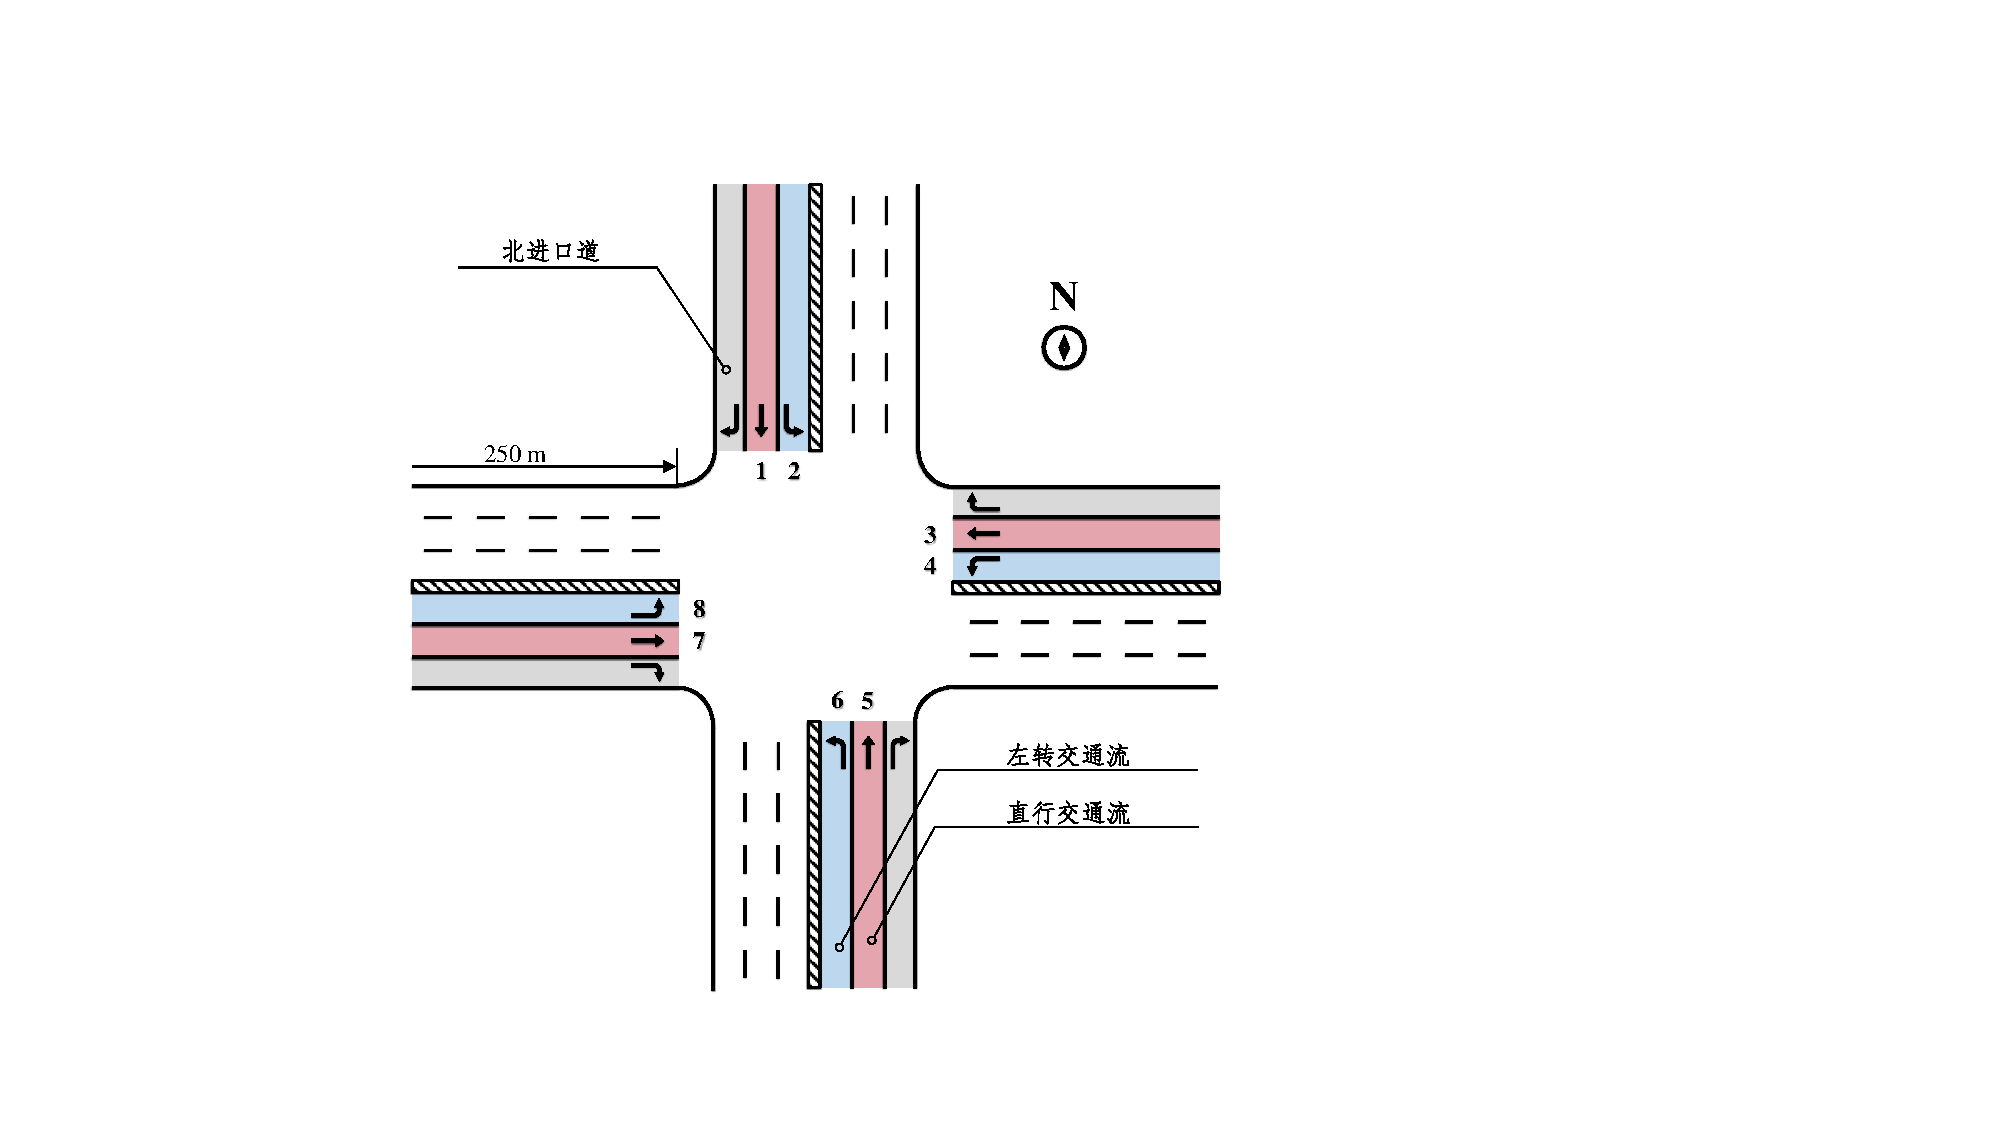
\includegraphics[width=0.9\textwidth,keepaspectratio]{intersection.pdf}
        \subcaption{交叉口交通组织}
        \label{fig:intersection}
    \end{minipage}
    \hfill % 在子图之间添加空格
    % 第二个子图
    \begin{minipage}[b]{.5\textwidth}
    \centering
        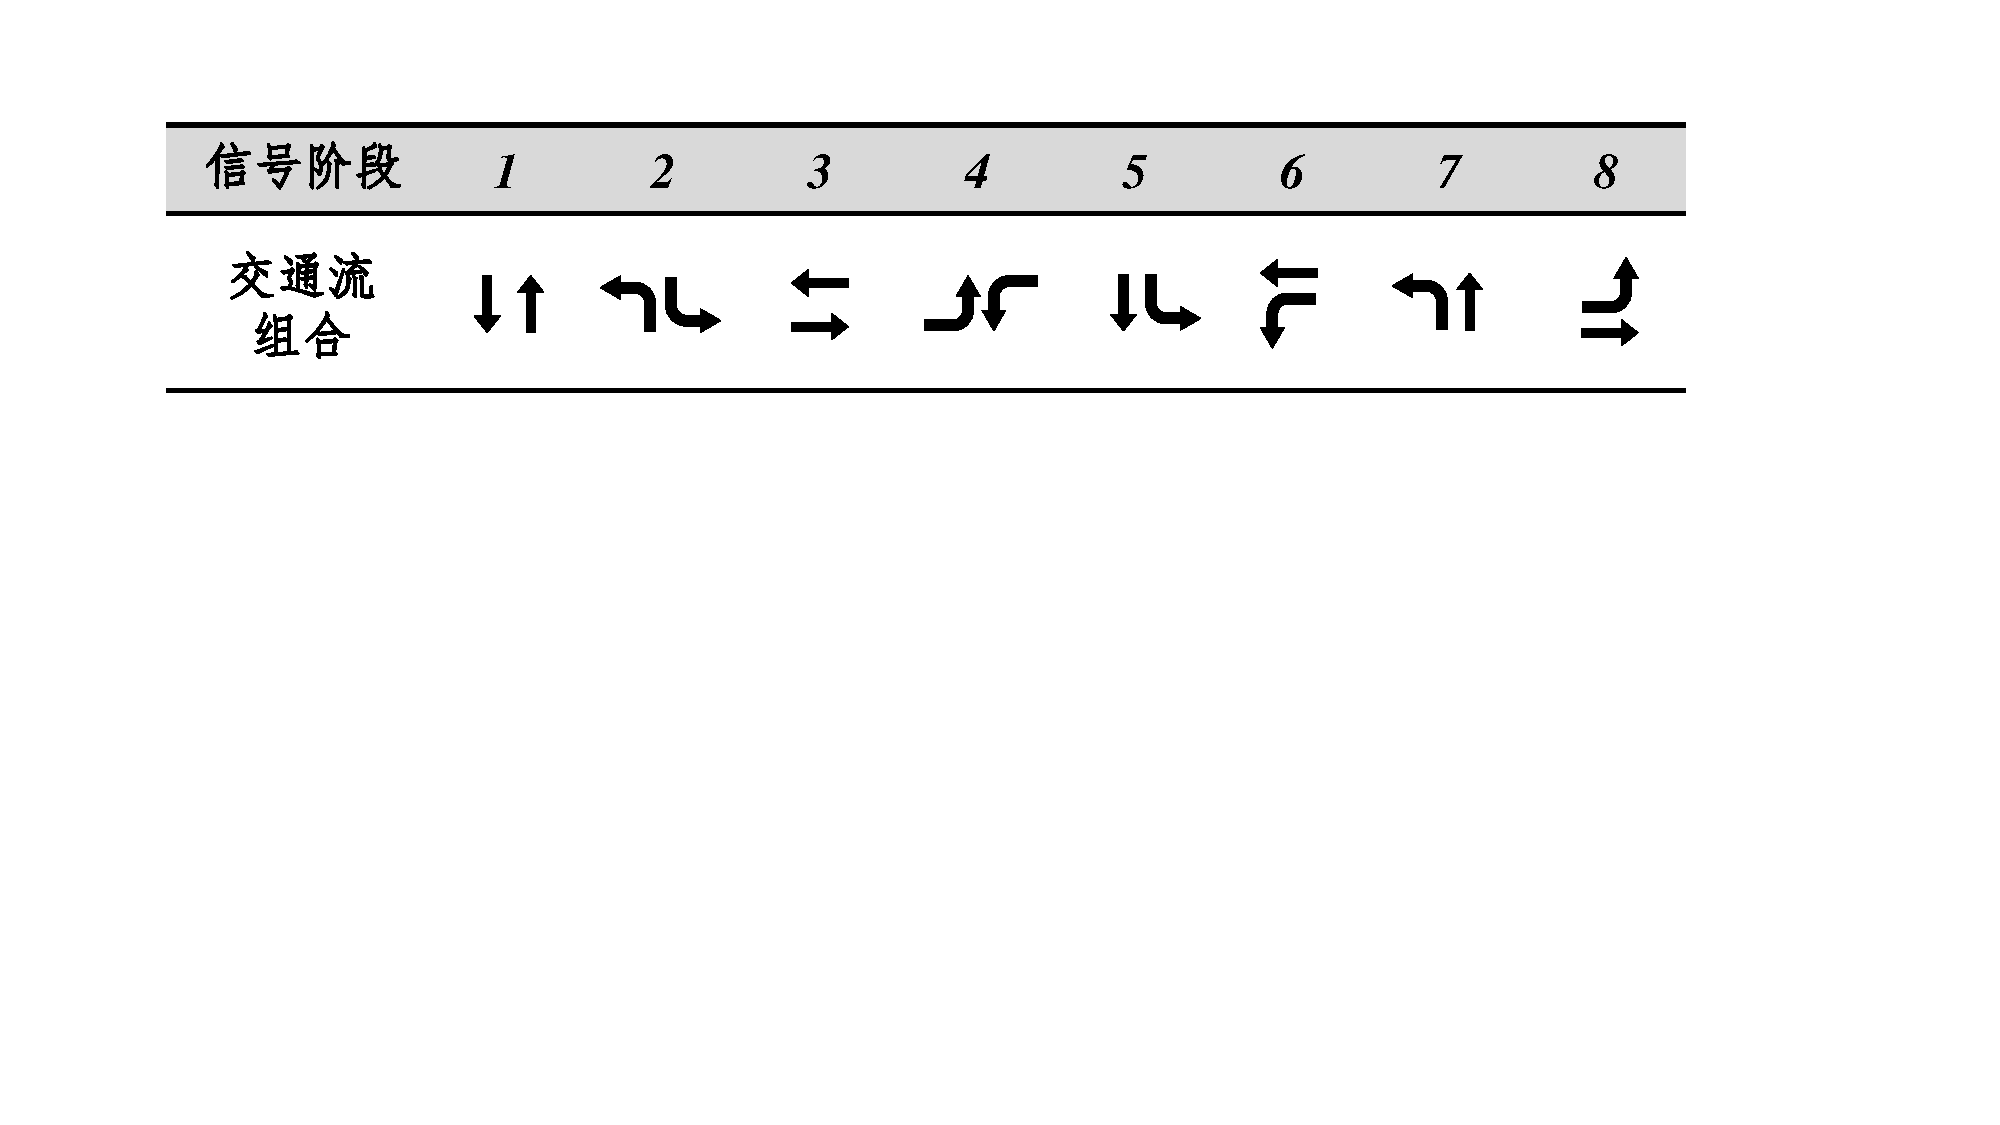
\includegraphics[width=0.9\textwidth,keepaspectratio]{movement_group.pdf}
        \subcaption{相位阶段}
        \label{fig:movement-groups}
        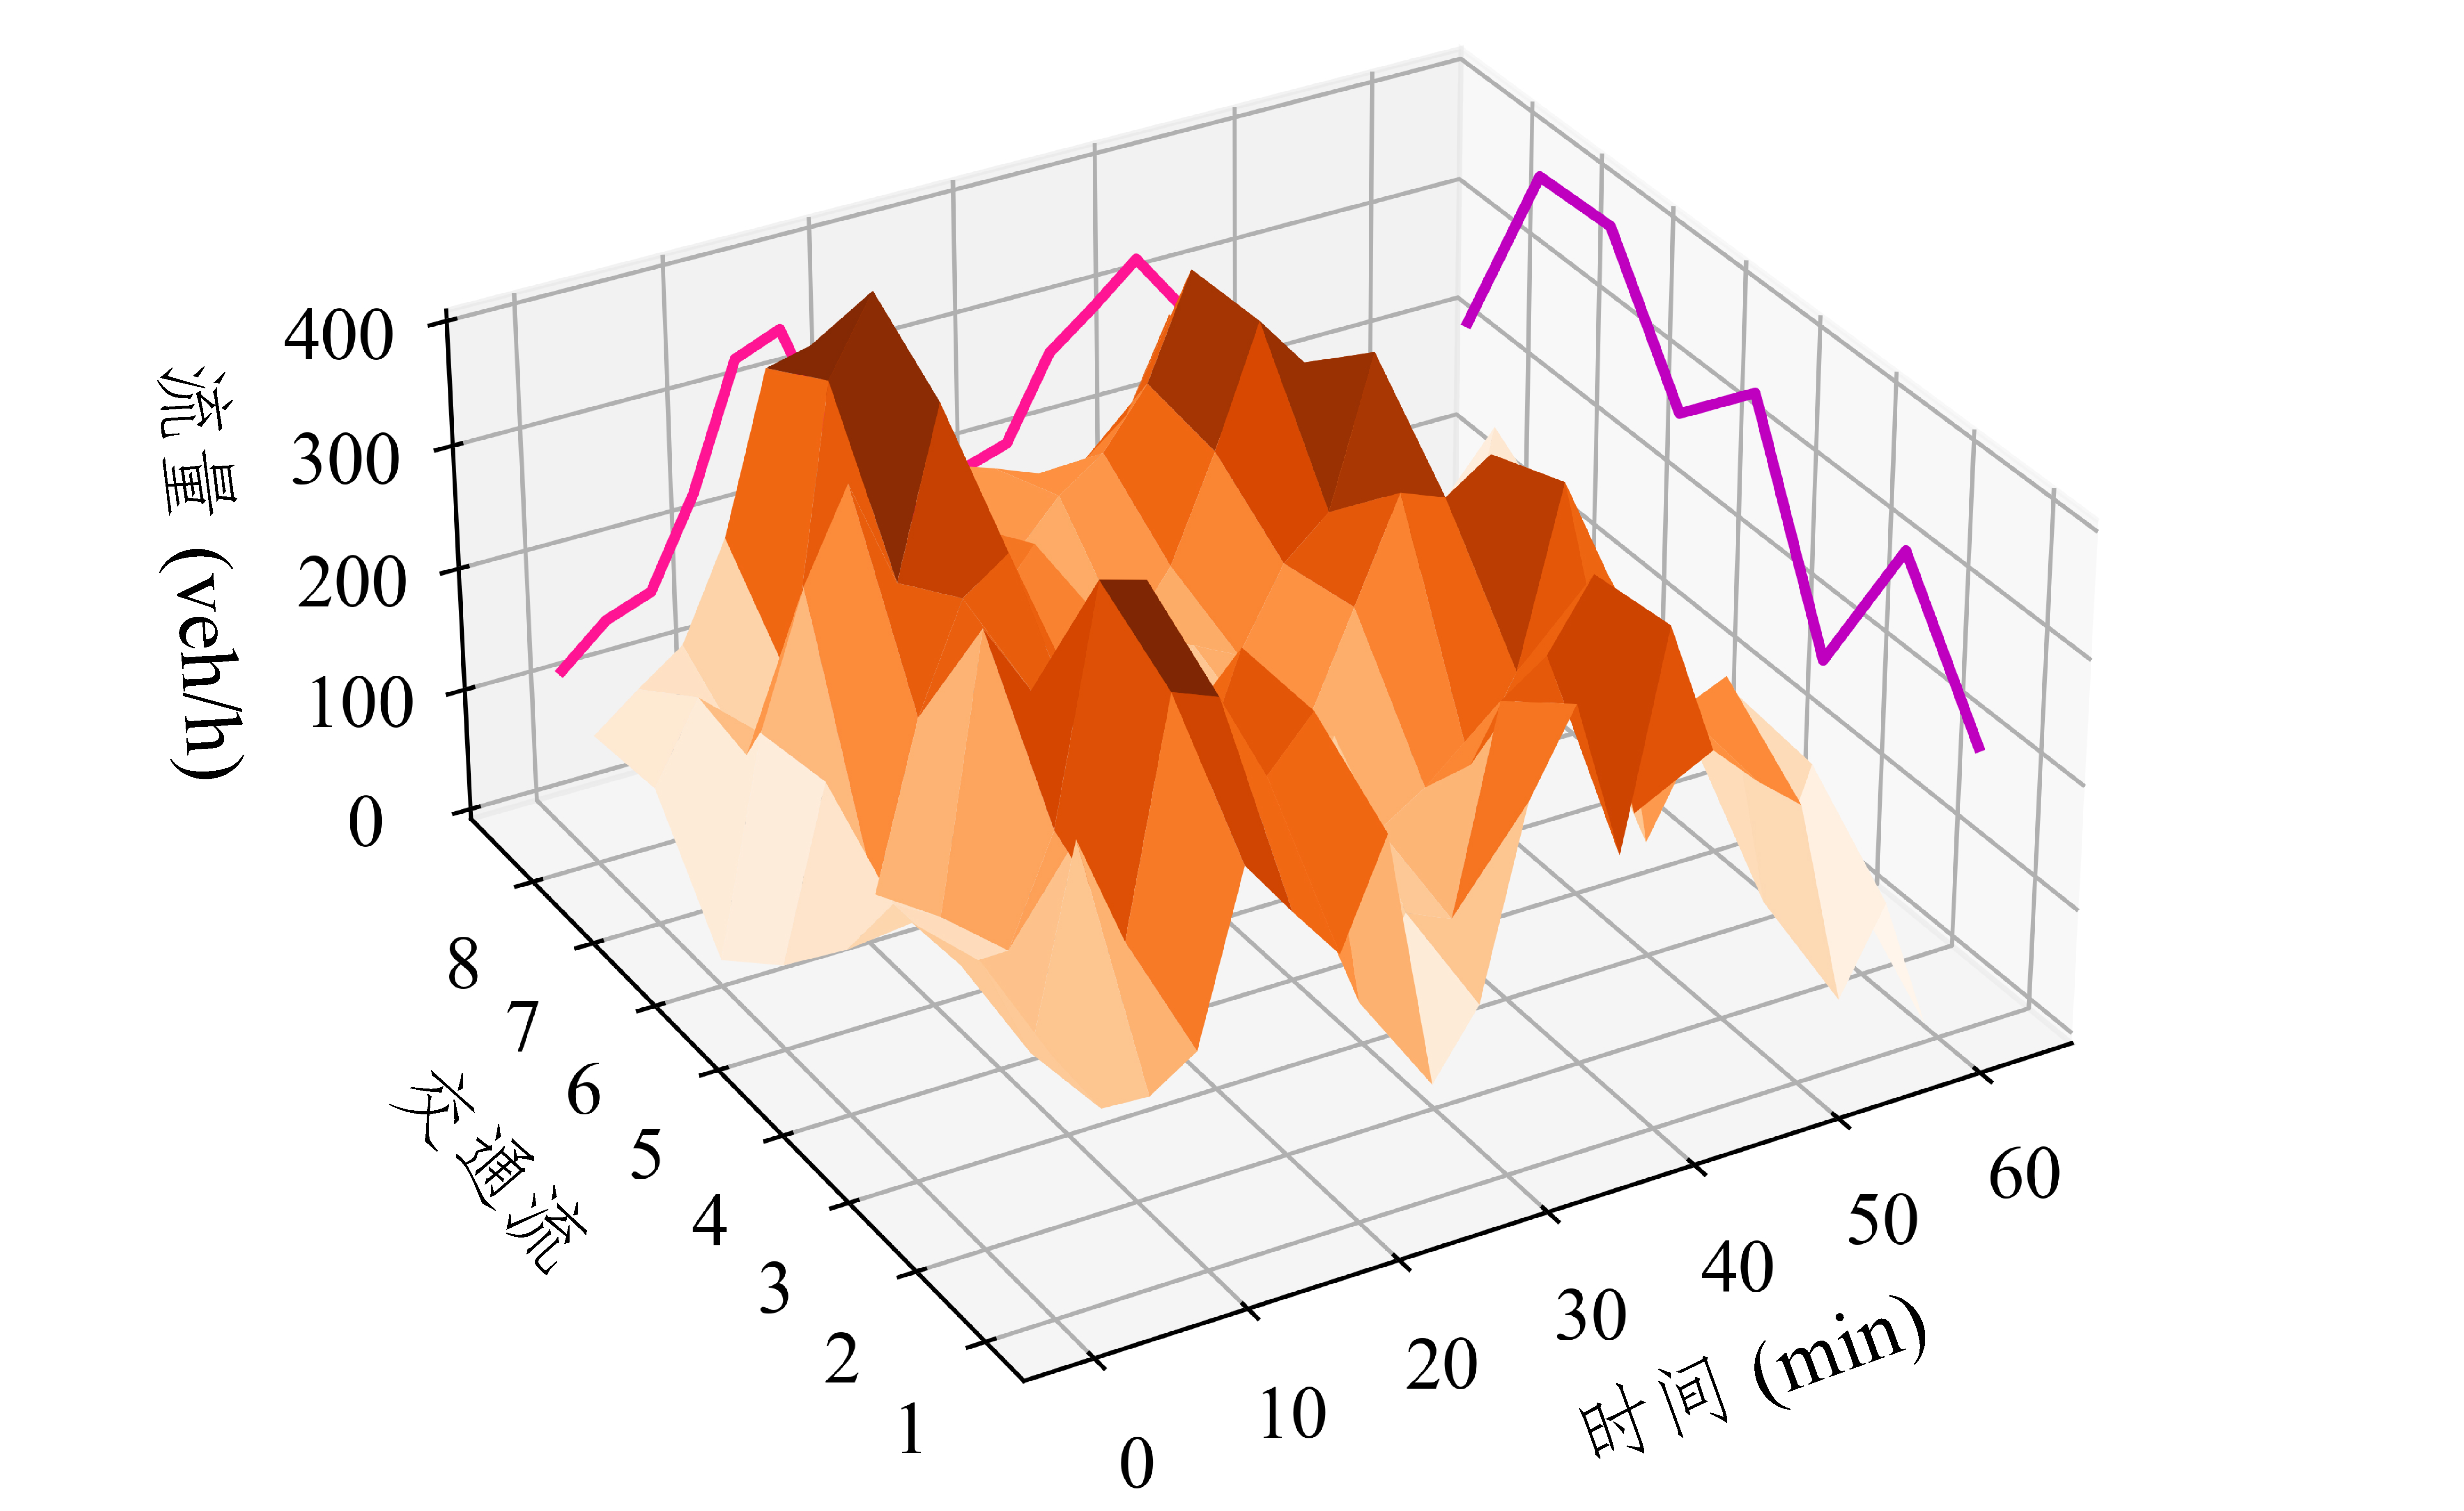
\includegraphics[width=0.95\textwidth,keepaspectratio]{oringinal_demand.pdf}
        \subcaption{一段时间内不同交通流所对应的交通需求}
        \label{fig:urban-traffic-demand}
    \end{minipage}
\caption{环境与交通需求示意图}
\label{fig:traffic-environment}    
\end{figure}

\begin{itemize}[leftmargin=*]
    \setlength{\itemsep}{0pt}
    \setlength{\parsep}{0pt}
    \setlength{\parskip}{0pt}

    
    \item \textbf{交通组织}。在仿真环境中每个交叉口都含有四个进口方向。如\Cref{fig:intersection} 所示,
    我们标记出了北进口道,该进口道设有三条车道,分别对应着左转、直行以及右转交通流。
    \item \textbf{交通流}。交通流是某股朝着特定方向行进的交通。如\Cref{fig:intersection} 所示,
    有八股交通流在信号灯的管控之下,但不包含右转交通流。通常情况下,右转交通流在任何条件下都可以通行,但其通行权优先级较低,必须让行于具有更高(通行权)优先级的冲突交通流。
    \item \textbf{信号阶段}。信号阶段是交叉口所有交通流通行权的一种组合形式。如\Cref{fig:movement-groups} 所示,
    与大多数现有工作只考虑了四个或甚至两个信号阶段不同,我们引入了八个信号阶段,以完全其所有的组合形式。
    \item \textbf{信号参数}。为了避免通行决策的困境,依据道路的限速,我们在每个信号阶段的末尾设置了三秒的黄灯信号。
    此外,为了避免在信号阶段切换过程中不同冲突交通流的潜在碰撞,我们引入了一秒的全红清空信号。
    每个信号阶段的最小绿灯时间为十秒,最大绿灯时间为四十五秒。
    \item \textbf{交通需求}。城市交通流作为人类行为的一种表现,在时间和空间上呈现出了显著的动态性。
    一方面,城市交通流的流量随时间波动,形成了所谓的“日间效应” (time-of-day effect) ;另一方面,
    在信号灯管控下的交通流往往呈现出被截断和不连续的状态,导致不同方向交通流流量的即时失衡。如\Cref{fig:urban-traffic-demand} 所示,为了阐明上述现象,同时也为了后续更好地揭示混合动作空间的潜在优势,我们在定义交通需求时引入了“时间不平衡性”与“方向不平衡性”两个关键概念。时间不平衡性,通过粉红色线条表示,描述了平均流量随时间的变化趋势;方向不平衡性,通过紫色线条表示,描述了任意时刻不同方向交通流间的不均衡状态。
\end{itemize}
\section{强化学习建模}
我们采用了深度强化学习(Deep Reinforcement Learning, DRL)来建模环境$\mathcal{E}$ 与智能体$\mathcal{G}$之间的交互,该算法受到了试错学习机制的启发。
在本研究中,假设智能体可以完整地获取交叉口的观测信息,并相应地调整信号灯时序;其最终目标是学习一种策略,以最小化最终目标。
具体而言,该过程可以被描述为一个马尔可夫决策过程(Markov Decision Process, MDP),记为$\prec \mathcal{S}, \mathcal{A}, \mathcal{P}, \mathcal{R}, \gamma\succ$ 。

给定状态空间$\mathcal{S}$与动作空间$\mathcal{A}$,奖励函数$\mathcal{R}$是从$\mathcal{S} \times \mathcal{A}$到$\mathbb{R}$的映射。智能体旨在学习一个最优策略
$\pi^\star(A_t = a | S_t = s)$,该策略根据当前状态确定最佳动作$a\thicksim\pi^\star(s)$,以最大化以下累积折扣回报:

\begin{equation}
    R_t = r_{t+1} + \gamma r_{t+2} + \gamma^2 r_{t+3} + \ldots = \sum_{k=0}^{\infty} \gamma^k r_{t+k+1}.
    \label{eq:total_discounted_return}
\end{equation}

鉴于本研究聚焦于混合动作空间,而非状态表征或奖励函数的设计,我们在随后的讨论中,将不会对后者展开详细的论述。事实上,不论是对于单点还是多点信号控制,
本文参考了现有研究[],采用了简单而有效的状态表征和奖励信号。具体地,其马尔可夫决策过程可被定义如下:


\begin{itemize}[leftmargin=*]
    \setlength{\itemsep}{0pt}
    \setlength{\parsep}{0pt}
    \setlength{\parskip}{0pt}

    
    \item \textbf{状态}:由每股交通流排队长度$q^{i}$拼接成的形状为$8\times1$的向量。其中,上标$i$表示第$i$股交通流;
    根据SUMO\footnote{参见SUMO的官方文档:\url{https://sumo.dlr.de/pydoc/traci._lane.html\#23LaneDomain-getLastStepHaltingNumber}}的定义,当车辆的速度小于0.1km/h时,车辆被定义为排队状态。
    \item \textbf{动作}:一个定义在混合动作空间$\mathcal{A}=\bigcup_{a\in\mathcal{A}_{d}}\{(a, x)|x\in\mathcal{X}_{a} \} $中的参数化动作$(a, x)$, 遵循[15]中的符号约定。
    其中,$a$是从信号阶段集合$\mathcal{A}_{d}=\{ a_{1}, a_{2}, ..., a_{8}\} $中选出的(离散的)信号阶段指示;而$\mathcal{X}_{a}\subseteq \mathbb{R} $是其相应的(连续的)参数,换句话说,该信号阶段所对应的绿灯时长。
    \item \textbf{奖励}:$\sum_{i=1}^{8} q^i_{t-1} - \sum_{i=1}^{8} q^i_{t}$, 上一时间步与当前时间步交叉口排队长度之差。
    
\end{itemize}

\section{基于SUMO的仿真引擎}




\chapter{再一章}

\par 如\autoref{alg:sample},这是一个算法

\begin{algorithm}[H]
    \begin{algorithmic} % enter the algorithmic environment
        \REQUIRE $n \geq 0 \vee x \neq 0$
        \ENSURE $y = x^n$
        \STATE $y \Leftarrow 1$
        \IF{$n < 0$}
            \STATE $X \Leftarrow 1 / x$
            \STATE $N \Leftarrow -n$
        \ELSE
            \STATE $X \Leftarrow x$
            \STATE $N \Leftarrow n$
        \ENDIF
        \WHILE{$N \neq 0$}
            \IF{$N$ is even}
                \STATE $X \Leftarrow X \times X$
                \STATE $N \Leftarrow N / 2$
            \ELSE[$N$ is odd]
                \STATE $y \Leftarrow y \times X$
                \STATE $N \Leftarrow N - 1$
            \ENDIF
        \ENDWHILE
    \end{algorithmic}
    \caption{\label{alg:sample}算法样例}
\end{algorithm}


\chapter{基于H-PPO算法的单点交通信号控制方法}
本章首先定义了交通环境$\mathcal{E}$ ,将其描述为一个独立的交叉口或涵盖众多交叉口的城市区段,其交通需求的生成结合了人工生成与实际采集的数据。
在上述交通环境中,我们部署了智能体$\mathcal{G}$ ,旨在通过实时调整交通信号的配时来优化交通流,以有效减轻交通拥堵。本研究基于SUMO开源仓库以及C++语言开发了仿真引擎,同时对于其并发性能进行了优化。
\section{引言}
\section{PPO算法简介}
\section{H-PPO算法简介与实现}
\section{仿真实验与分析}

\subsection{交通需求定义}
\subsection{实验基准设置}
\subsection{算法参数配置}
\subsection{实验结果与分析}

\section{本章小结}



\chapter{基于Hyar算法的单点交通信号控制方法}
本章首先定义了交通环境$\mathcal{E}$ ,将其描述为一个独立的交叉口或涵盖众多交叉口的城市区段,其交通需求的生成结合了人工生成与实际采集的数据。
在上述交通环境中,我们部署了智能体$\mathcal{G}$ ,旨在通过实时调整交通信号的配时来优化交通流,以有效减轻交通拥堵。本研究基于SUMO开源仓库以及C++语言开发了仿真引擎,同时对于其并发性能进行了优化。
\section{引言}
\section{VAE算法简介}
\section{Hyar算法简介与实现}
\section{仿真实验与分析}

\subsection{算法参数配置}
\subsection{实验结果与分析}
\subsection{混合动作空间机理揭示}

\section{本章小结}



\chapter{混合动作空间多智能体协作理论探究}
本章首先定义了交通环境$\mathcal{E}$ ,将其描述为一个独立的交叉口或涵盖众多交叉口的城市区段,其交通需求的生成结合了人工生成与实际采集的数据。
在上述交通环境中,我们部署了智能体$\mathcal{G}$ ,旨在通过实时调整交通信号的配时来优化交通流,以有效减轻交通拥堵。本研究基于SUMO开源仓库以及C++语言开发了仿真引擎,同时对于其并发性能进行了优化。
\section{引言}
\section{POMDPs与MacDec-POMDPs}
\section{不同范式下的策略更新理论}

\subsection{完全中心化}
\subsection{完全去中心化}
\subsection{中心化训练去中心化执行}

\section{仿真实验与分析}

\subsection{交通需求定义}
\subsection{实验基准设置}
\subsection{算法参数配置}
\subsection{实验结果与分析}

\section{本章小结}


\chapter{总结与展望}
本章首先定义了交通环境$\mathcal{E}$ ,将其描述为一个独立的交叉口或涵盖众多交叉口的城市区段,其交通需求的生成结合了人工生成与实际采集的数据。
在上述交通环境中,我们部署了智能体$\mathcal{G}$ ,旨在通过实时调整交通信号的配时来优化交通流,以有效减轻交通拥堵。本研究基于SUMO开源仓库以及C++语言开发了仿真引擎,同时对于其并发性能进行了优化。
\section{总结}
\section{展望}

